% A LaTeX template for MSc Thesis submissions to 
% Politecnico di Milano (PoliMi) - School of Industrial and Information Engineering
%
% S. Bonetti, A. Gruttadauria, G. Mescolini, A. Zingaro
% e-mail: template-tesi-ingind@polimi.it
%
% Last Revision: October 2021
%
% Copyright 2021 Politecnico di Milano, Italy. NC-BY

\documentclass{Configuration_Files/PoliMi3i_thesis}
\usepackage{minted}
\usepackage{textcomp}
\usepackage{xcolor}
\usepackage{listings}
\usepackage{upquote}
\definecolor{keyword}{HTML}{2771a3}
\definecolor{pattern}{HTML}{b53c2f}
\definecolor{string}{HTML}{be681c}
\definecolor{relation}{HTML}{7e4894}
\definecolor{variable}{HTML}{107762}
\definecolor{comment}{HTML}{8d9094}
\lstset{
	numbers=none,
	stepnumber=1,
	numbersep=5pt,
	basicstyle=\small\ttfamily,
	keywordstyle=\color{keyword}\bfseries\ttfamily,
	commentstyle=\color{comment}\ttfamily,
	stringstyle=\color{string}\ttfamily,
	identifierstyle=,
	showstringspaces=false,
	aboveskip=3pt,
	belowskip=3pt,
	columns=flexible,
	keepspaces=true,
	breaklines=true,
	captionpos=b,
	tabsize=2,
	frame=none,
}

\lstset{upquote=true}
\lstdefinelanguage{cypher}
{
	morekeywords={
		CALL, YIELD, ON, MATCH, OPTIONAL, WHERE, NOT, AND, OR, XOR, RETURN, DISTINCT, ORDER, BY, ASC, ASCENDING, DESC, DESCENDING, UNWIND, AS, UNION, WITH, ALL, CREATE, DELETE, DETACH, REMOVE, SET, MERGE, SET, SKIP, LIMIT, IN, CASE, WHEN, THEN, ELSE, END,
		INDEX, DROP, UNIQUE, CONSTRAINT, EXPLAIN, PROFILE, START, COUNT, IS, NULL
	}
}
\newcommand{\mycdots}{\cdot\!\cdot\!\cdot}
\lstset{language=cypher,
	literate=*
	{...}{$\mycdots$}{1}
	{theta}{$\theta$}{1}
}

%------------------------------------------------------------------------------
%	REQUIRED PACKAGES AND  CONFIGURATIONS
%------------------------------------------------------------------------------

% CONFIGURATIONS
\usepackage{parskip} % For paragraph layout
\usepackage{setspace} % For using single or double spacing
\usepackage{emptypage} % To insert empty pages
\usepackage{multicol} % To write in multiple columns (executive summary)
\setlength\columnsep{15pt} % Column separation in executive summary
\setlength\parindent{0pt} % Indentation
\raggedbottom  

% PACKAGES FOR TITLES
\usepackage{titlesec}
% \titlespacing{\section}{left spacing}{before spacing}{after spacing}
\titlespacing{\section}{0pt}{3.3ex}{2ex}
\titlespacing{\subsection}{0pt}{3.3ex}{1.65ex}
\titlespacing{\subsubsection}{0pt}{3.3ex}{1ex}
\usepackage{color}

% PACKAGES FOR LANGUAGE AND FONT
\usepackage[english]{babel} % The document is in English  
\usepackage[utf8]{inputenc} % UTF8 encoding
\usepackage[T1]{fontenc} % Font encoding
\usepackage[11pt]{moresize} % Big fonts

% PACKAGES FOR IMAGES
\usepackage{graphicx}
\usepackage{transparent} % Enables transparent images
\usepackage{eso-pic} % For the background picture on the title page
\usepackage{subfig} % Numbered and caption subfigures using \subfloat.
\usepackage{tikz} % A package for high-quality hand-made figures.
\usetikzlibrary{}
\graphicspath{{./Images/}} % Directory of the images
\usepackage{caption} % Coloured captions
\usepackage{xcolor} % Coloured captions
\usepackage{amsthm,thmtools,xcolor} % Coloured "Theorem"
\usepackage{float}

% STANDARD MATH PACKAGES
\usepackage{amsmath}
\usepackage{amsthm}
\usepackage{amssymb}
\usepackage{amsfonts}
\usepackage{bm}
\usepackage[overload]{empheq} % For braced-style systems of equations.
\usepackage{fix-cm} % To override original LaTeX restrictions on sizes

% PACKAGES FOR TABLES
\usepackage{tabularx}
\usepackage{longtable} % Tables that can span several pages
\usepackage{colortbl}

% PACKAGES FOR ALGORITHMS (PSEUDO-CODE)
\usepackage{algorithm}
\usepackage{algorithmic}

% PACKAGES FOR REFERENCES & BIBLIOGRAPHY
\usepackage[colorlinks=true,linkcolor=black,anchorcolor=black,citecolor=black,filecolor=black,menucolor=black,runcolor=black,urlcolor=black]{hyperref} % Adds clickable links at references
\usepackage{cleveref}
\usepackage[square, numbers, sort&compress]{natbib} % Square brackets, citing references with numbers, citations sorted by appearance in the text and compressed
\bibliographystyle{abbrvnat} % You may use a different style adapted to your field

% OTHER PACKAGES
\usepackage{pdfpages} % To include a pdf file
\usepackage{afterpage}
\usepackage{lipsum} % DUMMY PACKAGE
\usepackage{fancyhdr} % For the headers
\fancyhf{}

% Input of configuration file. Do not change config.tex file unless you really know what you are doing. 
% Define blue color typical of polimi
\definecolor{bluepoli}{cmyk}{0.4,0.1,0,0.4}

% Custom theorem environments
\declaretheoremstyle[
  headfont=\color{bluepoli}\normalfont\bfseries,
  bodyfont=\color{black}\normalfont\itshape,
]{colored}

% Set-up caption colors
\captionsetup[figure]{labelfont={color=bluepoli}} % Set colour of the captions
\captionsetup[table]{labelfont={color=bluepoli}} % Set colour of the captions
\captionsetup[algorithm]{labelfont={color=bluepoli}} % Set colour of the captions

\theoremstyle{colored}
\newtheorem{theorem}{Theorem}[chapter]
\newtheorem{proposition}{Proposition}[chapter]

% Enhances the features of the standard "table" and "tabular" environments.
\newcommand\T{\rule{0pt}{2.6ex}}
\newcommand\B{\rule[-1.2ex]{0pt}{0pt}}

% Pseudo-code algorithm descriptions.
\newcounter{algsubstate}
\renewcommand{\thealgsubstate}{\alph{algsubstate}}
\newenvironment{algsubstates}
  {\setcounter{algsubstate}{0}%
   \renewcommand{\STATE}{%
     \stepcounter{algsubstate}%
     \Statex {\small\thealgsubstate:}\space}}
  {}

% New font size
\newcommand\numfontsize{\@setfontsize\Huge{200}{60}}

% Title format: chapter
\titleformat{\chapter}[hang]{
\fontsize{50}{20}\selectfont\bfseries\filright}{\textcolor{bluepoli} \thechapter\hsp\hspace{2mm}\textcolor{bluepoli}{|   }\hsp}{0pt}{\huge\bfseries \textcolor{bluepoli}
}

% Title format: section
\titleformat{\section}
{\color{bluepoli}\normalfont\Large\bfseries}
{\color{bluepoli}\thesection.}{1em}{}

% Title format: subsection
\titleformat{\subsection}
{\color{bluepoli}\normalfont\large\bfseries}
{\color{bluepoli}\thesubsection.}{1em}{}

% Title format: subsubsection
\titleformat{\subsubsection}
{\color{bluepoli}\normalfont\large\bfseries}
{\color{bluepoli}\thesubsubsection.}{1em}{}

% Shortening for setting no horizontal-spacing
\newcommand{\hsp}{\hspace{0pt}}

\makeatletter
% Renewcommand: cleardoublepage including the background pic
\renewcommand*\cleardoublepage{%
  \clearpage\if@twoside\ifodd\c@page\else
  \null
  \AddToShipoutPicture*{\BackgroundPic}
  \thispagestyle{empty}%
  \if@twocolumn\hbox{}\fi\fi\fi}
\makeatother

%For correctly numbering algorithms
\numberwithin{algorithm}{chapter}

%----------------------------------------------------------------------------
%	NEW COMMANDS DEFINED
%----------------------------------------------------------------------------

% EXAMPLES OF NEW COMMANDS
\newcommand{\bea}{\begin{eqnarray}} % Shortcut for equation arrays
\newcommand{\eea}{\end{eqnarray}}
\newcommand{\e}[1]{\times 10^{#1}}  % Powers of 10 notation

%----------------------------------------------------------------------------
%	ADD YOUR PACKAGES (be careful of package interaction)
%----------------------------------------------------------------------------

%----------------------------------------------------------------------------
%	ADD YOUR DEFINITIONS AND COMMANDS (be careful of existing commands)
%----------------------------------------------------------------------------

%----------------------------------------------------------------------------
%	BEGIN OF YOUR DOCUMENT
%----------------------------------------------------------------------------

\begin{document}

\fancypagestyle{plain}{%
\fancyhf{} % Clear all header and footer fields
\fancyhead[RO,RE]{\thepage} %RO=right odd, RE=right even
\renewcommand{\headrulewidth}{0pt}
\renewcommand{\footrulewidth}{0pt}}

%----------------------------------------------------------------------------
%	TITLE PAGE
%----------------------------------------------------------------------------


\frontmatter % Use roman page numbering style (i, ii, iii, iv...) for the preamble pages

\puttitle{
	title=Systems and Methods for Big and Unstructured Data Project - First Delivery,
	name1= 1. Lorenzo Biasiolo - 10629367, % Author Name and Surname
	name2= 2. Grecya D'Angiò - 10651939, 
	name3= 3. Elia Maggioni - 10610008, 
	name4= 4. Enrico Maria Marinelli - 10898730,
	name5= 5. Carlos Santillán - 10659783,
	academicyear=2022-2023,
	groupnumber= 7
} 
% These info will be put into your Title page 

%----------------------------------------------------------------------------
%	PREAMBLE PAGES: ABSTRACT (inglese e italiano), EXECUTIVE SUMMARY
%----------------------------------------------------------------------------
\setcounter{page}{1} % Set page counter to 1

%----------------------------------------------------------------------------
%	LIST OF CONTENTS/FIGURES/TABLES/SYMBOLS
%----------------------------------------------------------------------------

% TABLE OF CONTENTS
\thispagestyle{empty}
\tableofcontents % Table of contents 
\thispagestyle{empty}
\cleardoublepage

%-------------------------------------------------------------------------
%	THESIS MAIN TEXT
%-------------------------------------------------------------------------
% In the main text of your thesis you can write the chapters in two different ways:
%
%(1) As presented in this template you can write:
%    \chapter{Title of the chapter}
%    *body of the chapter*
%
%(2) You can write your chapter in a separated .tex file and then include it in the main file with the following command:
%    \chapter{Title of the chapter}
%    \input{chapter_file.tex}
%
% Especially for long thesis, we recommend you the second option.

\addtocontents{toc}{\vspace{2em}} % Add a gap in the Contents, for aesthetics
\mainmatter % Begin numeric (1,2,3...) page numbering

\chapter{Introduction and project specification}
\label{ch:chapter_one}%
% The \label{...}% enables to remove the small indentation that is generated, always leave the % symbol.
\section{Problem description}
\label{sec:section_name}
This project aims to design and implement a computer science bibliography database. We are inspired mainly by the structure of the DBLP website, which is the current reference for accessing scientific articles and the bibliography in computer science. In addition, the system must be able to store scientific papers and books, their authors, and references of such works in a structured fashion, keep track of venues at which they have been presented and guarantee access to all relevant information for a scientific researcher. Lastly, the implementation uses a graph database, specifically Neo4j.

\section{Overlook of DBLP}
\label{sec:section_name}
DBLP is a computer science bibliography website. It lists over 5.4 million journal articles, conference papers, and other computer science publications. Among the most relevant information for our purposes are the following:

\begin{itemize}
\item Author information, including his/her affiliation.
\item Publication information, which can be an article or a book.
\item Citations and references of each publication.
\item Keywords or fields of study of each publication.
\item Related conferences / journals of each publication.
\item Authorship information (co-authors).
\item Publishers.
\end{itemize}

\section{Hypotheses}
\label{sec:section_name}
We made the following hypotheses:
\begin{itemize}
    \item An author can be affiliated to one and only one organization.
    \item There is no distinction between the authors of the same publication, no ranking nor order. We assume they all have contributed equally to the publication.
    \item A publication $X$ must cite at least one other publication, but it is admissible that no one has cited (referenced) $X$.
    \item There are no joint publishers (i.e., publishers that share publication rights for the publications). Each publication must have one and only one publisher (even if it is presented at a conference).
    \item Publications stored in the database can either be books or articles. No other types exist. It could eventually be expanded to include works like Ph.D. theses and independent publications.
    \item Each article must be presented in one venue regardless of the type of venue.
    \item A publication cannot reference itself.
    \item Whenever we see missing values in the dataset we set them to a default value.
\end{itemize}
\chapter{Conceptual model}
\label{ch:chapter_one}

%Figures, Tables and Algorithms have to contain a Caption that describe their content, and have to be properly reffered in the text.

\subsection{ER diagram}
\label{subsec:figures}

An entity–relationship model (or ER model) describes interrelated subjects of interest in a specific knowledge domain. A basic ER model is composed of entity types and specifies relationships that can exist between entities.

In this case, we have created a general ER for a bibliographic database. We consider the following entities:
\begin{itemize}
\item \textbf{Publication}: The core entity of the dataset, represents any published document of any of the allowed types. Attributes:
\begin{itemize}
      \item \textit{\textbf{IDP}}: Primary key of the publication, it is different from the DOI and the ISBN.
      \item \textit{Title}: Title of the publication.
      \item \textit{Year}: Year of publication.
      \item \textit{Pages}: Number of pages of publication.
      \item \textit{Abstract}: Abstract of the publication.
    \end{itemize}
\item \textbf{Field of Study}:  an area in which the publication is awarded.Attributes:
\begin{itemize}
    \item \textit{\textbf{ISBN}}: Primary key, the International Standard Book Number.
\end{itemize}
\item \textbf{Book}: Type of publication (inherits Publication entity) that models books. Attributes:
\begin{itemize}
    \item \textit{\textbf{Name}}: Primary key, the field of study's name.
\end{itemize}
\item \textbf{Article}: Type of publication (inherits Publication entity) that models articles, these are published at a venue. Attributes:
\begin{itemize}
    \item \textit{\textbf{DOI}}: Primary key, Document Object Identifier.
\end{itemize}
\item \textbf{Author}: Authors that write publications. Attributes:
\begin{itemize}
      \item \textit{\textbf{IDA}}: Primary key, it emulates the ORCID.
      \item \textit{Name}: The author's name.
    \end{itemize}
\item \textbf{Field of Study}: A specific field of study that is covered by publications, it substitutes the keywords. Attributes:
\begin{itemize}
      \item \textit{\textbf{Name}}: Name of the publication. 
\end{itemize}
\item \textbf{Organization}: An organization to which authors are affiliated. Attributes:
\begin{itemize}
      \item \textit{\textbf{IDO}}: Primary key, unique ID.
      \item \textit{Name}: Name of the organization.
      \item \textit{Address}: Main address of the organization.
\end{itemize}
\item \textbf{Publisher}: An entity that publishes articles and books.
\begin{itemize}
      \item \textit{\textbf{IDP}}: Primary key, unique ID.
      \item \textit{Name}: Name of the publisher. 
      \item \textit{Address}: Main address of the publisher.
\end{itemize}
\item \textbf {Venue}: Venue at which the articles are published 
\begin{itemize}
      \item\textit{\textbf{ID}}: Primary key, unique ID.
      \item \textit{Name}: Name of the venue. 
    \end{itemize}

\item \textbf {Journal}: A scientific journal (inherits Venue entity). Attributes:
\begin{itemize}
     \item \textit{Volume}: A certain volume of the journal.
\end{itemize}
\item \textbf {Conference}: A scientific conference (inherits Venue entity). Attributes:
\begin{itemize}
      \item \textit{Place}: Location where the conference takes place.
      \item \textit{Data interval}: Days in which the conference takes place.
    \end{itemize}
\end{itemize}

\textit{Note on cardinality}:

To avoid any ambiguity, here is an example how to read cardinalities in our ER diagram. 

An author (left) is affiliated to one and only one organization (right) and at least one author or more must be affiliated to any given organization.

\begin{figure}[H]
    \centering
    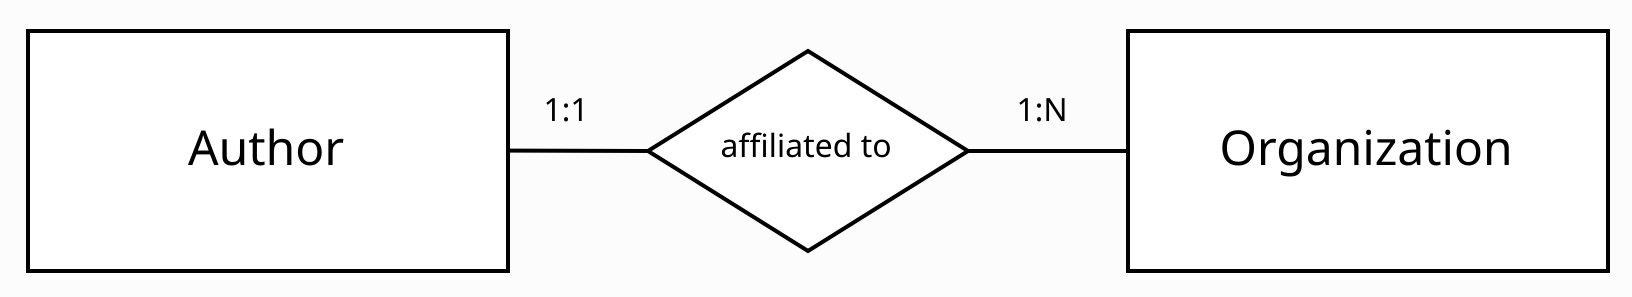
\includegraphics[width=0.4\textwidth]{Images/legenda.png}
    \caption{Cardinality legend}
    \label{fig:quadtree}
\end{figure}
\begin{figure}[H]
    \centering
    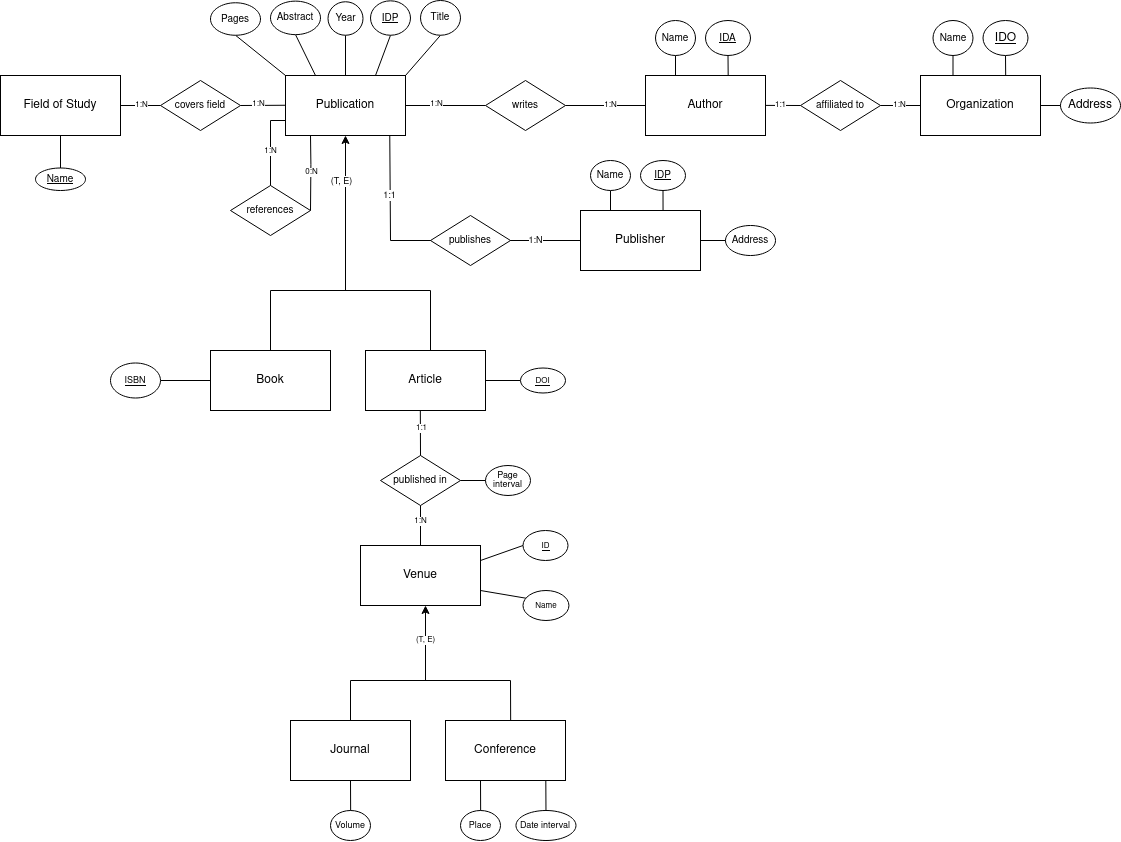
\includegraphics[width=170mm, height = 170mm, scale = 1]{Images/ER1.png}
    \caption{ER diagram.}
    \label{fig:quadtree}
\end{figure}

\chapter{Graph diagram}
\section{Description of graph diagram}
The graph diagram is the following.
\begin{figure}[H]
    \centering
    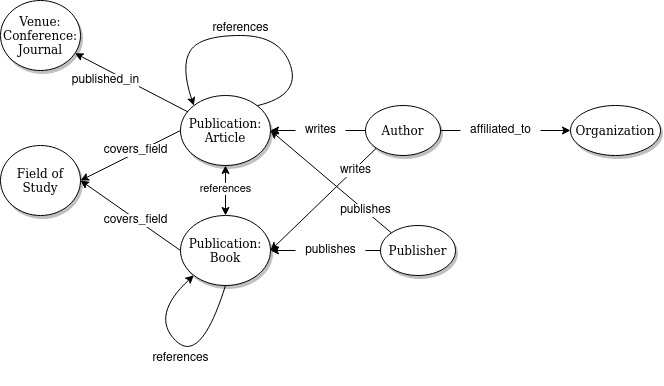
\includegraphics[width=1\textwidth]{Images/graph.drawio.png}
    \caption{Graph diagram}
    \label{fig:quadtree}
\end{figure}
There is an almost perfect correspondence with the ER diagram except for a few key differences. Any node with the \textit{Publication} label may also have the label \textit{Article} or \textit{Book} (but not both); it represents the hierarchy seen in the ER. Publications with the label \textit{Article} are be published in a venue (which can have different attributes depending on the subsequent label \textit{Conference} or \textit{Journal}). However \textit{Book} does not; hence we see a distinction in the diagram above. 

Notice that a publication may reference any other publications regardless of the type. In general any node with the \textit{Publication} label may reference at least one \textit{Publication} node, be written by at least one \textit{Author}, published by a \textit{Publisher} and cover at least one \textit{Field of Study}.
\section{Description of nodes}
In this section we describe each node and its properties. Note that \textit{page\_start} and \textit{page\_end} indicate the interval in the journal/proceedings where the article is located. The citations property refers to a past citation count and is recomputed whenever necessary.
\begin{itemize}
    \item \textbf{Publication}:
    \begin{itemize}
        \item \textit{id}: Integer
        \item \textit{page\_start}: Integer
        \item \textit{page\_end}: Integer
        \item \textit{pages}: Integer (the number of pages)
        \item \textit{title}: String
        \item \textit{year}: Integer
        \item \textit{citations}: Integer
    \end{itemize}
    \item \textbf{Publication:Article}:
    \begin{itemize}
        \item \textit{DOI}: String 
    \end{itemize}
    \item \textbf{Publication:Book}:
    \begin{itemize}
        \item \textit{ISBN}: String
    \end{itemize}
    \item \textbf{Author}:
    \begin{itemize}
        \item \textit{id}: Integer
        \item \textit{name}: String
    \end{itemize}
    \item \textbf{Publisher}:
    \begin{itemize}
        \item \textit{name}: String
    \end{itemize}
    \item \textbf{Organization}:
    \begin{itemize}
        \item \textit{name}: String
    \end{itemize}
    \item \textbf{Field of Study}: 
    \begin{itemize}
        \item \textit{name}: String
    \end{itemize}
    \item \textbf{Venue}: 
    \begin{itemize}
        \item \textit{name}: String
    \end{itemize}
\end{itemize}
The relationships are the ones shown in Figure 3.1. As we said before, a publication may refer to any number of publications (excluding itself). The \texttt{published\_in} relationship may occur only between nodes of type \texttt{Publication:Article} and not \texttt{Publication:Book}. For every other purpose, they share the same relationships. \\
Full list of relationships:
\begin{itemize}
    \item \texttt{references}: May occur between any two nodes with the \texttt{Publication} label.
    \item \texttt{writes}: Between nodes \texttt{Author} and \texttt{Publication}.
    \item \texttt{publishes}: Between \texttt{Publisher} and \texttt{Publication}.
    \item \texttt{affiliated\_to}: Between \texttt{Author} and \texttt{Organization}.
    \item \texttt{covers\_field}: Between \texttt{Publication} and \texttt{Field of Study}.
    \item \texttt{published\_in}: Between a node of label \texttt{Publication:Article} and a node of label \texttt{Venue} (regardless of sublabel \texttt{Conference} or \texttt{Journal}). 
\end{itemize}
\begin{figure}[H]
    \centering
    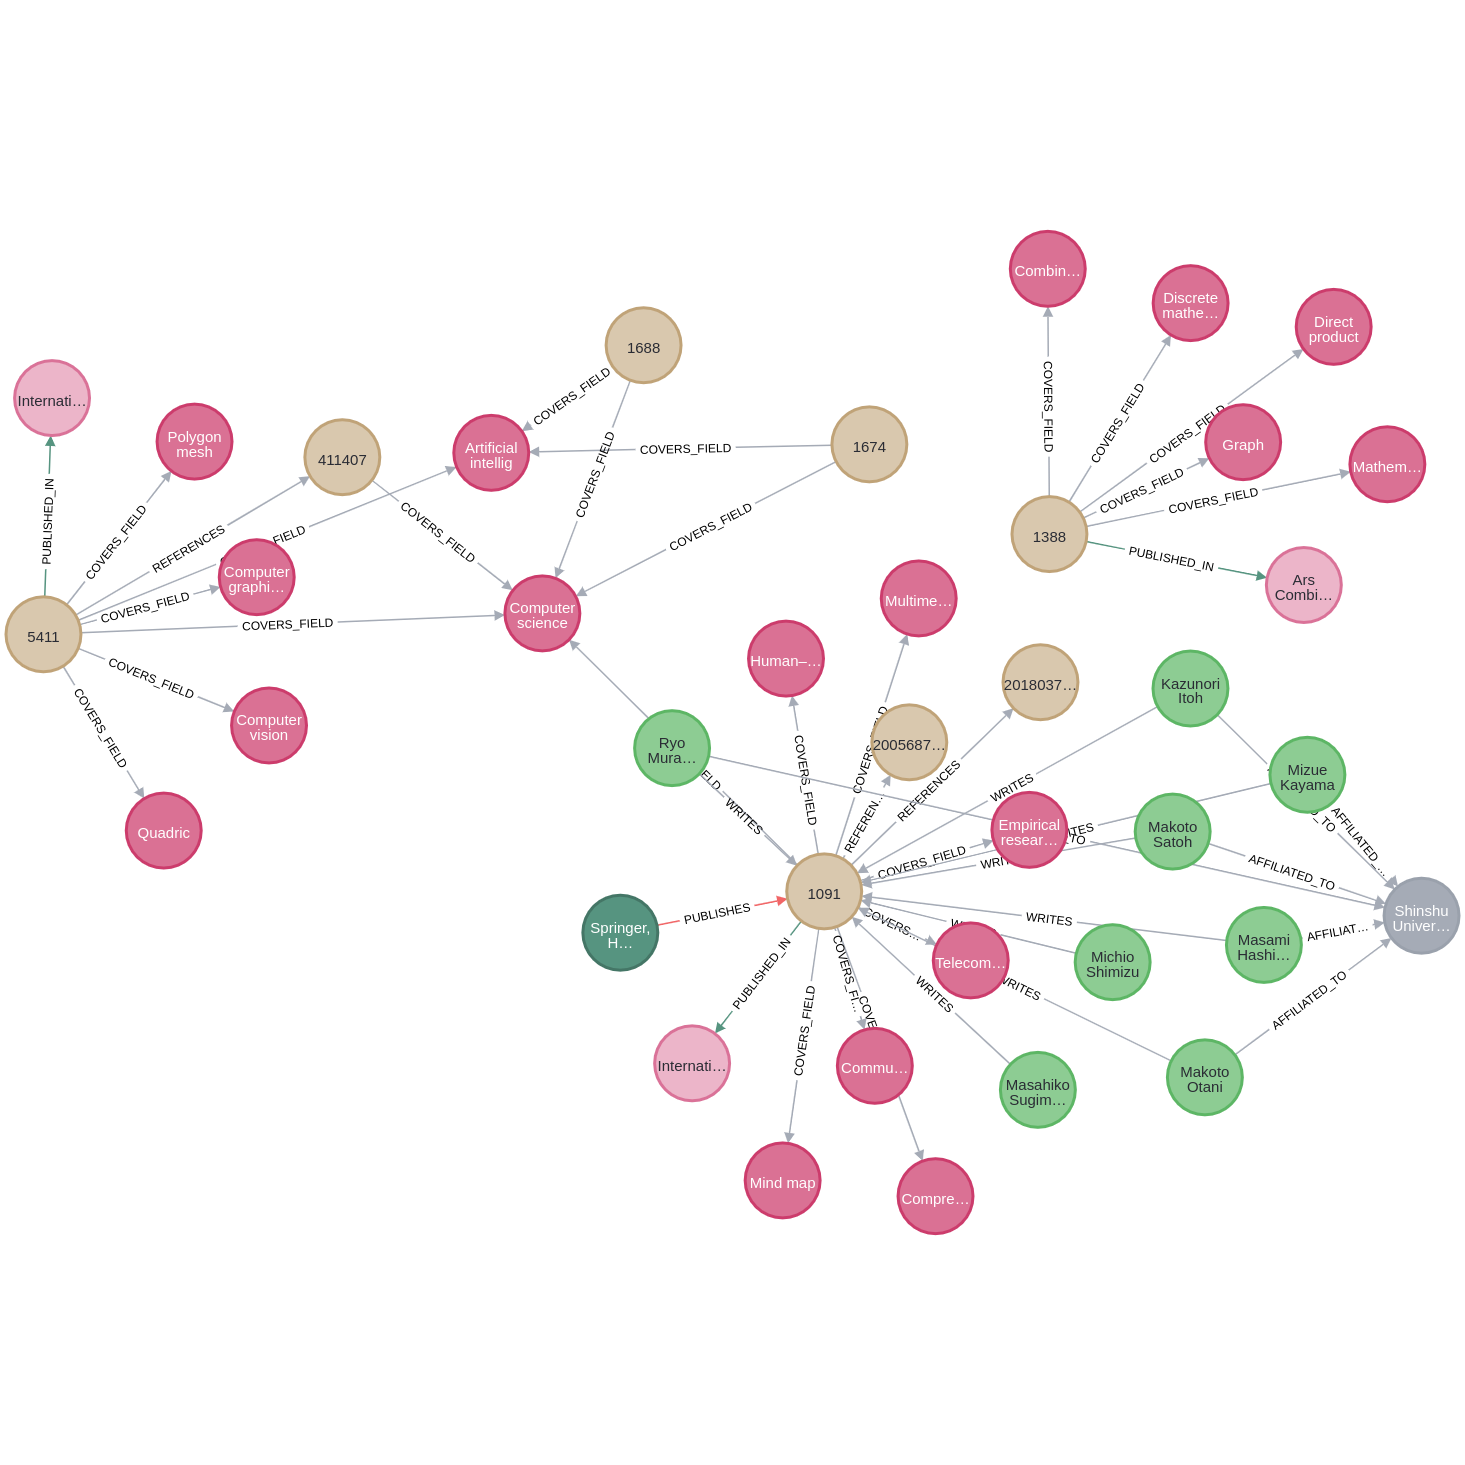
\includegraphics[width=1\textwidth]{Images/graph.png}
    \caption{Graph sample}
    \label{fig:quadtree}
\end{figure}
\chapter{Dataset description and import}
\label{ch:chapter_one}%
\section{Description of the dataset}
The dataset had a .json format and had the following structure for each item.
\begin{verbatim}
[
    {
        "id": 2456,
        "authors": [{"name": "Mario Rossi", "id": 4, 
                     "org": "Politecnico di Milano"}],
        "title": "Non-cooperative games",
        "abstract": "This is an awesome report, here is why"
        "year": 2005,
        "page_start": 245,
        "page_end": 255,
        "doc_type": "article",
        "publisher": "Springer",
        "fields": [{"name": "Computer science"}, 
                   {"name": "Artificial intelligence"}],
        "venue": {"raw": "Game theory journal", "id": 235, "type": "J"}
    }
    {
        "id": 2453
        ...
        ...
    }
    ...
]
\end{verbatim}
An item is a publication of some type. It has a title, id, authors, publishers, fields covered, and venue (if any).
\section{Data import into Neo4j}
The following scripts were used to import the entire dataset into the graph structure presented in Chapter 3.
\subsection{Initial upload of articles, main nodes and relationships}
This Cypher script uploads the main types of nodes, such as Articles, Publishers, Authors, Fields of Study, and their relationships.\\
\begin{lstlisting}[language=cypher, label=lst:cypher-example]
//1_load_articles_authors
CALL apoc.load.json("file:///articles_and_books.json") YIELD value AS 
entry
WHERE entry.doc_type <> "Book"
MERGE (p:Article:Publication {id:entry.id})
ON CREATE SET p.title = entry.title, p.year = entry.year, p.citations = entry.n_citation, 
p.page_start = entry.page_start, p.page_end = entry.page_end, 
p.pages = toInteger(entry.page_end) - toInteger(entry.page_start),
p.abstract = entry.abstract,
p.doi = randomUUID()
MERGE (pub:Publisher {name:entry.publisher})
MERGE (pub)-[:PUBLISHES]-(p)
MERGE (v:Venue {name:entry.venue.raw})
MERGE (p)-[:PUBLISHED_IN]->(v)
WITH p, entry
UNWIND entry.fos AS fos
MERGE (f:FieldOfStudy {name:fos.name})
MERGE (p)-[:COVERS_FIELD]->(f)
WITH p, entry
UNWIND entry.references AS reference
MERGE (ref:Publication {id:reference})
MERGE (p)-[:REFERENCES]->(ref)
WITH p, entry.authors AS authors
UNWIND authors AS author
MERGE (a:Author {id:author.id})
ON CREATE SET a.name = author.name
MERGE (a)-[:WRITES]->(p);
\end{lstlisting}
As usual, we use the \texttt{MERGE} command to avoid creating unwanted duplicates. We see that first, we upload all rows (publications) of a type different from Book (which we consider to be articles by default). The Book publications were scarce and had to be found beyond the first 2000 rows of the file and subsequently appended. We capture the relationships \texttt{COVERS\_FIELD}, \texttt{REFERENCES}, \texttt{WRITES}, \texttt{PUBLISHES} and \texttt{PUBLISHED\_IN}. The APOC library was necessary to correctly read the .json format.
\subsection{Books upload}
It is the same script from before, but this time the condition is that the document type is \textit{Book} and the operations concerning a Venue are omitted.
\subsection{Affiliations upload}
We upload the affiliations of each author. \\
\begin{lstlisting}[language=cypher, label=lst:cypher-example]
CALL apoc.load.json("file:///articles_and_books.json") YIELD value AS 
entry
WITH entry.authors AS authors
UNWIND authors AS author
MATCH (a:Author {id:author.id})
WHERE author.org IS NOT NULL
MERGE (aff:Organization {name:author.org})
MERGE (a)-[:AFFILIATED_TO]->(aff);
\end{lstlisting}
\subsection{Venue type setting upload}
We set the type of venue according to the \textit{type} value. \\
\begin{lstlisting}[language=cypher, label=lst:cypher-example]
CALL apoc.load.json("file:///articles_and_books.json") YIELD value AS 
entry
WHERE entry.doc_type <> "Book"
MATCH (v:Venue {name:entry.venue.raw})
WITH v,entry.venue as venue
WHERE venue.type = 'J'
SET v:Journal;
\end{lstlisting}
The rest of venues are assumed to be conferences.
\begin{lstlisting}[language=cypher, label=lst:cypher-example]
CALL apoc.load.json("file:///articles_and_books.json") YIELD value AS 
entry
WHERE entry.doc_type <> "Book"
MATCH (v:Venue {name:entry.venue.raw})
WITH v
WHERE not "Journal" in labels(v)
SET v:Conference;
\end{lstlisting}
We also added random citations to compensate the sparsity of a matrix.
\chapter{Queries and data creation}
\label{ch:chapter_one}%
\section{Data creation commands}
We present 5 data creation commands.
\subsection{Create an article}
Creation of a simple article. In practice, it is immediately followed by a relationship with its references, authors, etc. It cannot remain disconnected; otherwise, it would be coherent with the cardinalities of the ER diagram.
\\
\begin{lstlisting}[language=cypher, label=lst:cypher-example]
CREATE (p:Publication:Article {id: 123, name: 'SMBUD report', year: 2022})
\end{lstlisting}
\begin{figure}[H]
    \centering
    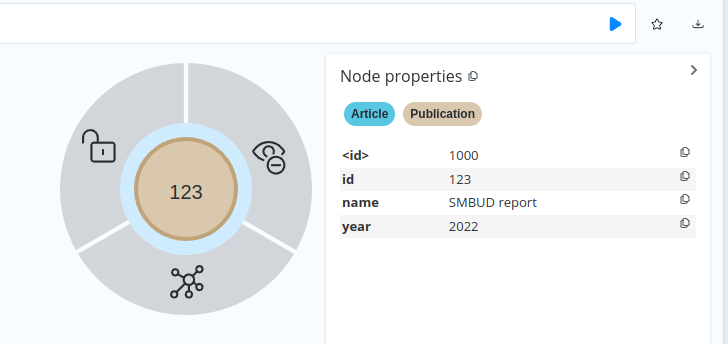
\includegraphics[width=100mm, height=50mm]{Images/create_1.png}
    \caption{}
    \label{fig:quadtree}
\end{figure}
\subsection{Add a field of study to an article}
We update the fields of the article with \textit{id} equal to 123.\\\\
\begin{lstlisting}[language=cypher, label=lst:cypher-example]
MATCH (p:Publication {id:123}) 
MATCH (f:FieldOfStudy {name: 'Computer science'})
CREATE (p)-[:COVERS_FIELD]->(f)
\end{lstlisting}
\begin{figure}[H]
    \centering
    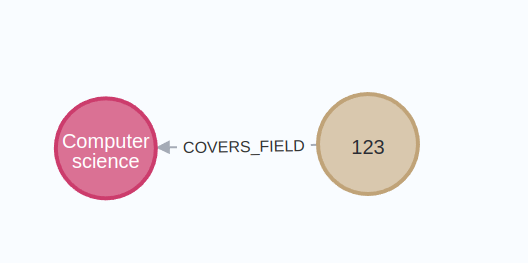
\includegraphics[width=100mm, height=50mm]{Images/create_2.png}
        \caption{}
    \label{fig:quadtree}
\end{figure}
\subsection{Add the authors of a certain article}
We add the authors of the article with \textit{id} 123.\\
\begin{lstlisting}[language=cypher, label=lst:cypher-example]
MATCH (p:Publication {id:123})
CREATE (a1:Author {id:25, name: 'John Smith'})
CREATE (a2:Author {id:26, name: 'Joan Smith'})
CREATE (a1)-[:WRITES]->(p)
CREATE (a2)-[:WRITES]->(p)
\end{lstlisting}
\begin{figure}[H]
    \centering
    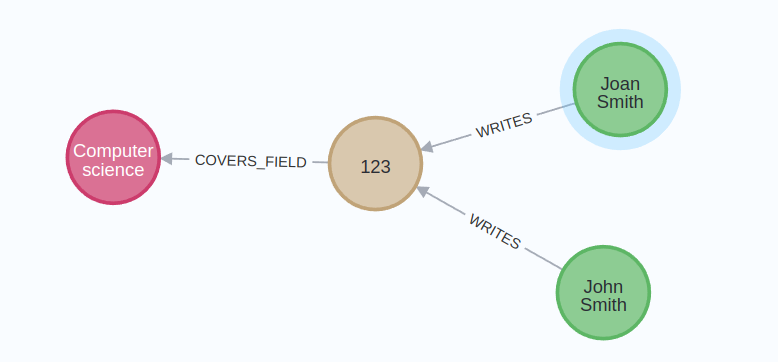
\includegraphics[width=100mm, height=50mm]{Images/create_3.png}
        \caption{}
    \label{fig:quadtree}
\end{figure}
\subsection{Create the affiliations of the authors of an article}
We create the affiliations of the article with \textit{id} equal to 123. Both authors will have the same affiliation.\\https://www.overleaf.com/project/63506d20dee2f339bb0b1b59
\begin{lstlisting}[language=cypher, label=lst:cypher-example]
MATCH (p:Article {id:123})
CREATE (o:Organization {name:"Imaginary University"})
WITH p, o
MATCH (a:Author)-[:WRITES]->(p)
CREATE (a)-[:AFFILIATED_TO]->(o)
\end{lstlisting}
\begin{figure}[H]
    \centering
    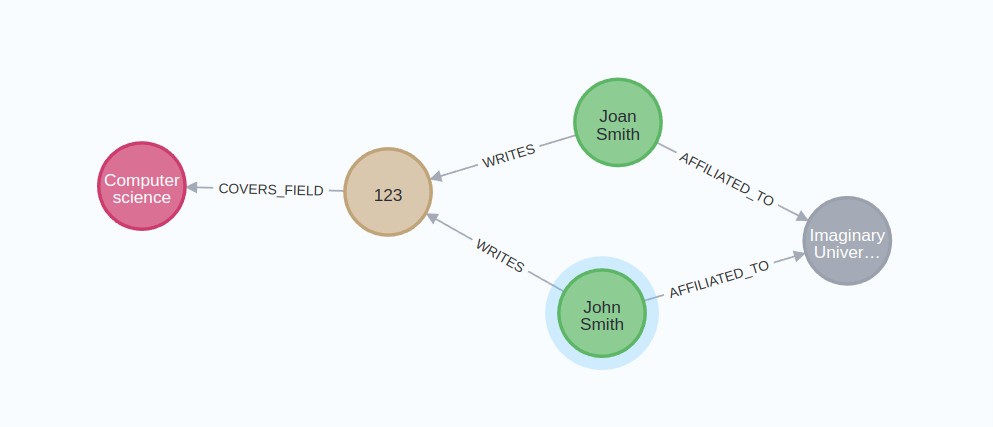
\includegraphics[width=100mm, height=50mm]{Images/create_4.png}
        \caption{}
    \label{fig:quadtree}
\end{figure}
\subsection{Change properties of an article}
We change the name of the article seen before.\\
\begin{lstlisting}[language=cypher, label=lst:cypher-example]
MATCH(p:Article {id:123})
SET p.name = 'SMBUD Neo4j', p.year = 2020
\end{lstlisting}
\begin{figure}[H]
    \centering
    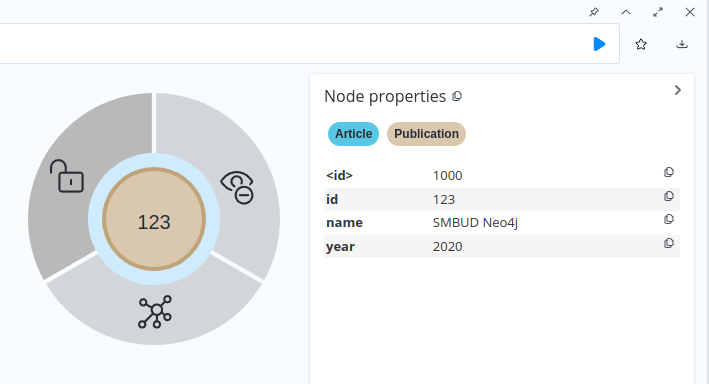
\includegraphics[width=100mm, height=50mm]{Images/create_5.png}
        \caption{}
    \label{fig:quadtree}
\end{figure}
\section{Queries}
In this section, we present a mix of queries ranging from simple to more elaborate.
\subsection{Find affiliations of authors who have written articles in a specific conference} 
We choose the conference named \textit{European Society for Fuzzy Logic and Technology Conference}. Since we chose the first 2000 lines and added random citations, it is natural that the results are sparse.\\
\begin{lstlisting}[language=cypher, label=lst:cypher-example]
MATCH (o:Organization) <-[:AFFILIATED_TO]-(:Author)-[:WRITES]->(:Article)-[:PUBLISHED_IN]->(c:Conference)
WHERE c.name = 'European Society for Fuzzy Logic and Technology Conference'
RETURN DISTINCT o
\end{lstlisting}
\begin{figure}[H]
    \centering
    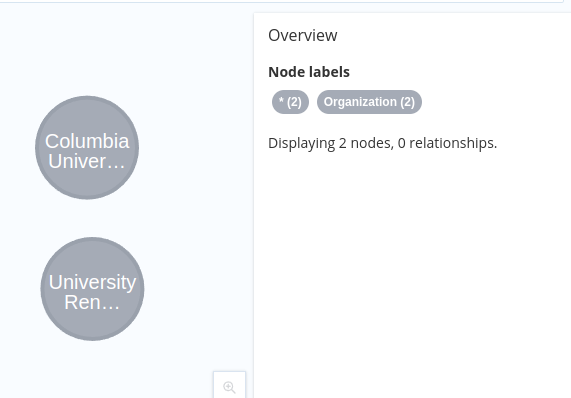
\includegraphics[width=100mm, height=50mm]{Images/query_1.png}
        \caption{}
    \label{fig:quadtree}
\end{figure}
\subsection{Find number of publications (covering a specific field and with at least 10 pages) published in conferences per year}
In this case we consider the field of computer science.\\
\begin{lstlisting}[language=cypher, label=lst:cypher-example]
MATCH (p:Publication)-[:COVERS_FIELD]->(:FieldOfStudy {name:'Computer science'})
WITH DISTINCT p.year AS years
UNWIND years AS y
MATCH (:FieldOfStudy {name:'Computer science'})<-[:COVERS_FIELD]-(p:Publication {year:y})-[:PUBLISHED_IN]->(:Conference)
WHERE p.pages >= 10
WITH COUNT(p) AS publications, y
ORDER BY y DESC
RETURN collect({number_of_publications:publications, year:y})
\end{lstlisting}
\begin{figure}[H]
    \centering
    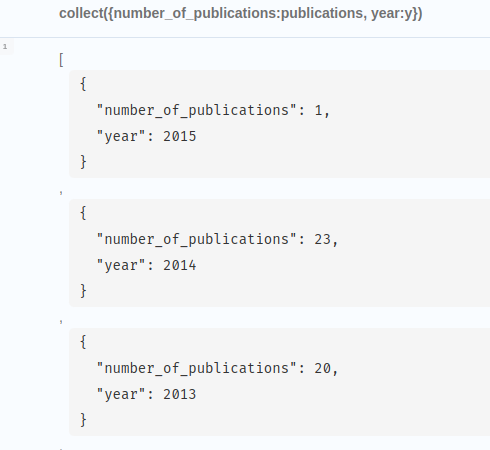
\includegraphics[width=80mm,height=50mm]{Images/query_2.png}
        \caption{}
    \label{fig:quadtree}
\end{figure}
\subsection{Find conference publications with at least 5 citations (references) by a publication written within the next 5 years of the original publication year}
\begin{lstlisting}[language=cypher, label=lst:cypher-example]
MATCH (:Conference)<-[:PUBLISHED_IN]-(p:Publication)<-[r:REFERENCES]-(q:Publication)
WHERE (q.year - p.year) <= 5
WITH COUNT(r) AS citations, p
WHERE citations >= 5
RETURN p
\end{lstlisting}
\begin{figure}[H]
    \centering
    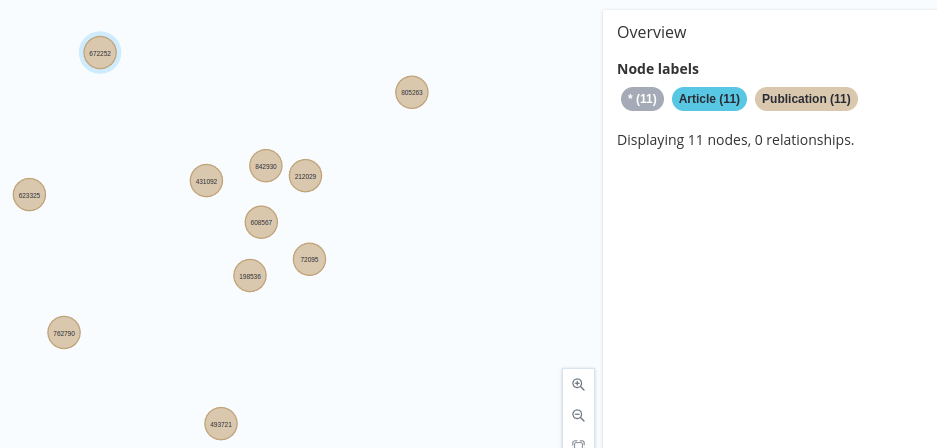
\includegraphics[width=100mm, height=63mm]{Images/query_3.png}
        \caption{}
    \label{fig:quadtree}
\end{figure}
\subsection{Find the top 5 organizations whose authors have written the most articles (with at least 10 pages) in the field of Computer Science}
\begin{lstlisting}[language=cypher, label=lst:cypher-example]
MATCH (f:FieldOfStudy {name:'Computer science'})<-[c:COVERS_FIELD]-(a:Article)<-[:WRITES]-(:Author)-[:AFFILIATED_TO]->(o:Organization)
WHERE a.pages >= 10
WITH DISTINCT o, c
WITH COUNT(c) AS articles, o
ORDER BY articles DESC
LIMIT 5
RETURN collect({organization:o.name, articles:articles})
\end{lstlisting}
\begin{figure}[H]
    \centering
    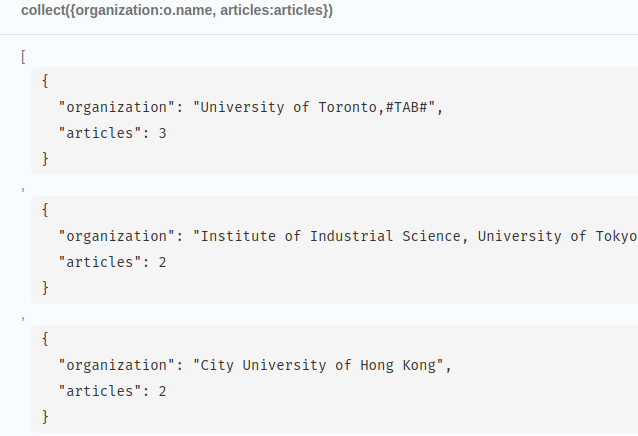
\includegraphics[width=100mm,height=50mm]{Images/query_4.png}
        \caption{}
    \label{fig:quadtree}
\end{figure}
\subsection{Find the venue(s) with the most articles related to Artificial Intelligence, must include not only the name but the number of articles as well}
Here we initially find the maximum number of articles, match the pattern and count again. We compare the count with the maximum value because there than one venue the same number of articles related to AI. We could also try to order the first results according to the number of articles and return the top-K venues; however, we have to know a priori the number of venues.\\
\begin{lstlisting}[language=cypher, label=lst:cypher-example]
MATCH (f:FieldOfStudy {name:'Artificial intelligence'})<-[:COVERS_FIELD]-(:Article)-[p:PUBLISHED_IN]->(v:Venue)
WITH COUNT(p) AS articles, v
WITH MAX(articles) AS max
MATCH (f:FieldOfStudy {name:'Artificial intelligence'})<-[:COVERS_FIELD]-(:Article)-[p:PUBLISHED_IN]->(v:Venue)
WITH COUNT(p) AS articles, v, max
WHERE articles = max
RETURN collect({venue:v.name, articles:articles})
\end{lstlisting}
\begin{figure}[H]
    \centering
        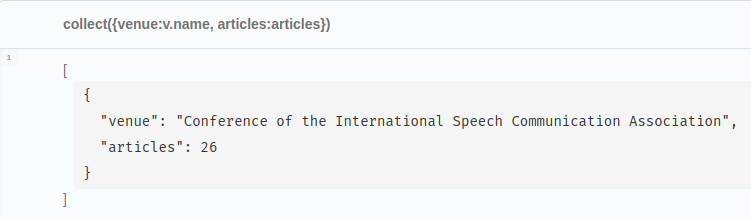
\includegraphics[width=85mm, height=50mm]{Images/query_5.png}
        \caption{}
    \label{fig:quadtree}
\end{figure}
\subsection{Find the pair(s) of publications (written after 2005) that share the highest amount of fields covered}
To avoid considering the same pair twice we simply add the condition $id1 > id2$. This way we only consider each unique combination once (and ignore the pair order).\\
\begin{lstlisting}[language=cypher, label=lst:cypher-example]
MATCH (p1:Publication)-[:COVERS_FIELD]->(f:FieldOfStudy)<-[:COVERS_FIELD]-(p2:Publication)
WHERE p1.year >= 2005 AND p2.year >= 2005 AND p1.id > p2.id
WITH COUNT(f) AS common_fields, p1, p2
WITH MAX(common_fields) AS max_fields
MATCH (p1:Publication)-[:COVERS_FIELD]->(f:FieldOfStudy)<-[:COVERS_FIELD]-(p2:Publication)
WHERE p1.year >= 2005 AND p2.year >= 2005
WITH COUNT(f) AS common_fields, p1, p2, max_fields
WHERE common_fields = max_fields AND p1.id > p2.id
RETURN collect({common_fields:common_fields, p1:p1.title, p2:p2.title})
\end{lstlisting}
\begin{figure}[H]
    \centering
    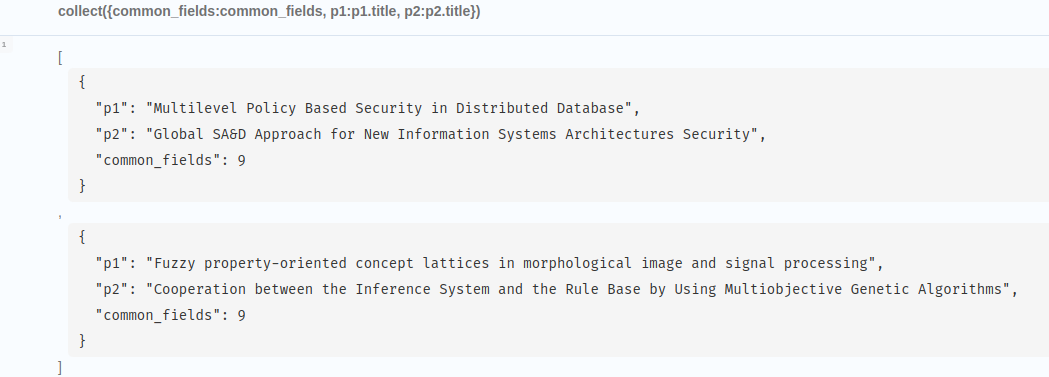
\includegraphics[width=100mm, height=50mm]{Images/query_7.png}
        \caption{}
    \label{fig:quadtree}
\end{figure}
\subsection{Find the average number of references made by conference articles covering a specific field written by authors affiliated with a certain organization}
We consider the field of computer science and the organization \textit{Karadeniz Technical Univ.}\\
\begin{lstlisting}[language=cypher, label=lst:cypher-example]
MATCH (o:Organization)<-[:AFFILIATED_TO]-(:Author)-[:WRITES]->(p:Publication)-[:PUBLISHED_IN]->(:Conference)
MATCH (p)-[:COVERS_FIELD]->(f:FieldOfStudy)
MATCH (p)-[r:REFERENCES]->(:Publication)
WHERE f.name = 'Computer science' AND o.name = 'Karadeniz Technical Univ.'
WITH COUNT(DISTINCT r) AS references, p
RETURN AVG(references) AS average_number_of_references
\end{lstlisting}
\begin{figure}[H]
    \centering
    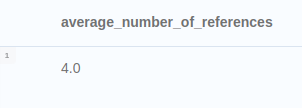
\includegraphics[width=80mm, height=50mm]{Images/query_6.png}
        \caption{}
    \label{fig:quadtree}
\end{figure}
\subsection{Find the top 3 publishers by number of published conference articles (who must reference at least 10 other publications) covering a specific field}

\begin{lstlisting}[language=cypher, label=lst:cypher-example]
MATCH (:Publication)<-[r:REFERENCES]-(a:Article)-[:COVERS_FIELD]->(:FieldOfStudy {name:'Computer science'})
MATCH (a)-[:PUBLISHED_IN]->(:Conference)
WITH COUNT(r) AS references, a
WHERE references >= 10
MATCH (publisher:Publisher)-[publishes:PUBLISHES]->(a)
WITH COUNT(publishes) AS articles, publisher
ORDER BY articles DESC LIMIT 3
RETURN collect({articles:articles, publisher:publisher.name})
\end{lstlisting}
\begin{figure}[H]
    \centering
    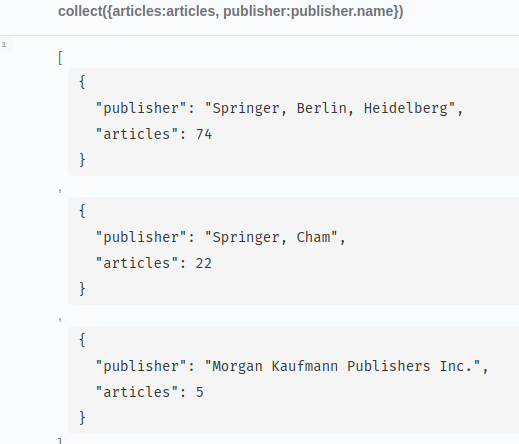
\includegraphics[width=80mm, height=50mm]{Images/query_8.png}
        \caption{}
    \label{fig:quadtree}
\end{figure}
\subsection{Find the articles (with at least 12 pages) that cover the most fields by the publisher who has published the most articles}
In this case, we consider the publisher who appears first in the sorted list; there may be different publishers with the same number of publications. However, in this case,  we limit ourselves to the first one we find.\\
\begin{lstlisting}[language=cypher, label=lst:cypher-example]
MATCH (publisher:Publisher)-[pub:PUBLISHES]->(:Article)
WITH COUNT(pub) AS publications, publisher
ORDER BY publications DESC LIMIT 1
WITH publisher
MATCH (publisher)-[:PUBLISHES]->(a:Article)-[c:COVERS_FIELD]->(:FieldOfStudy)
WHERE a.pages >= 12
WITH COUNT(c) AS fields, a, publisher
WITH MAX(fields) AS max_fields, publisher
MATCH (publisher)-[:PUBLISHES]->(a:Article)-[c:COVERS_FIELD]->(:FieldOfStudy)
WITH COUNT(c) AS fields, a, max_fields
WHERE fields = max_fields AND a.pages >= 12
RETURN a
\end{lstlisting}
Figure 5.11 shows the connected nodes as well (for context).
\begin{figure}[H]
    \centering
    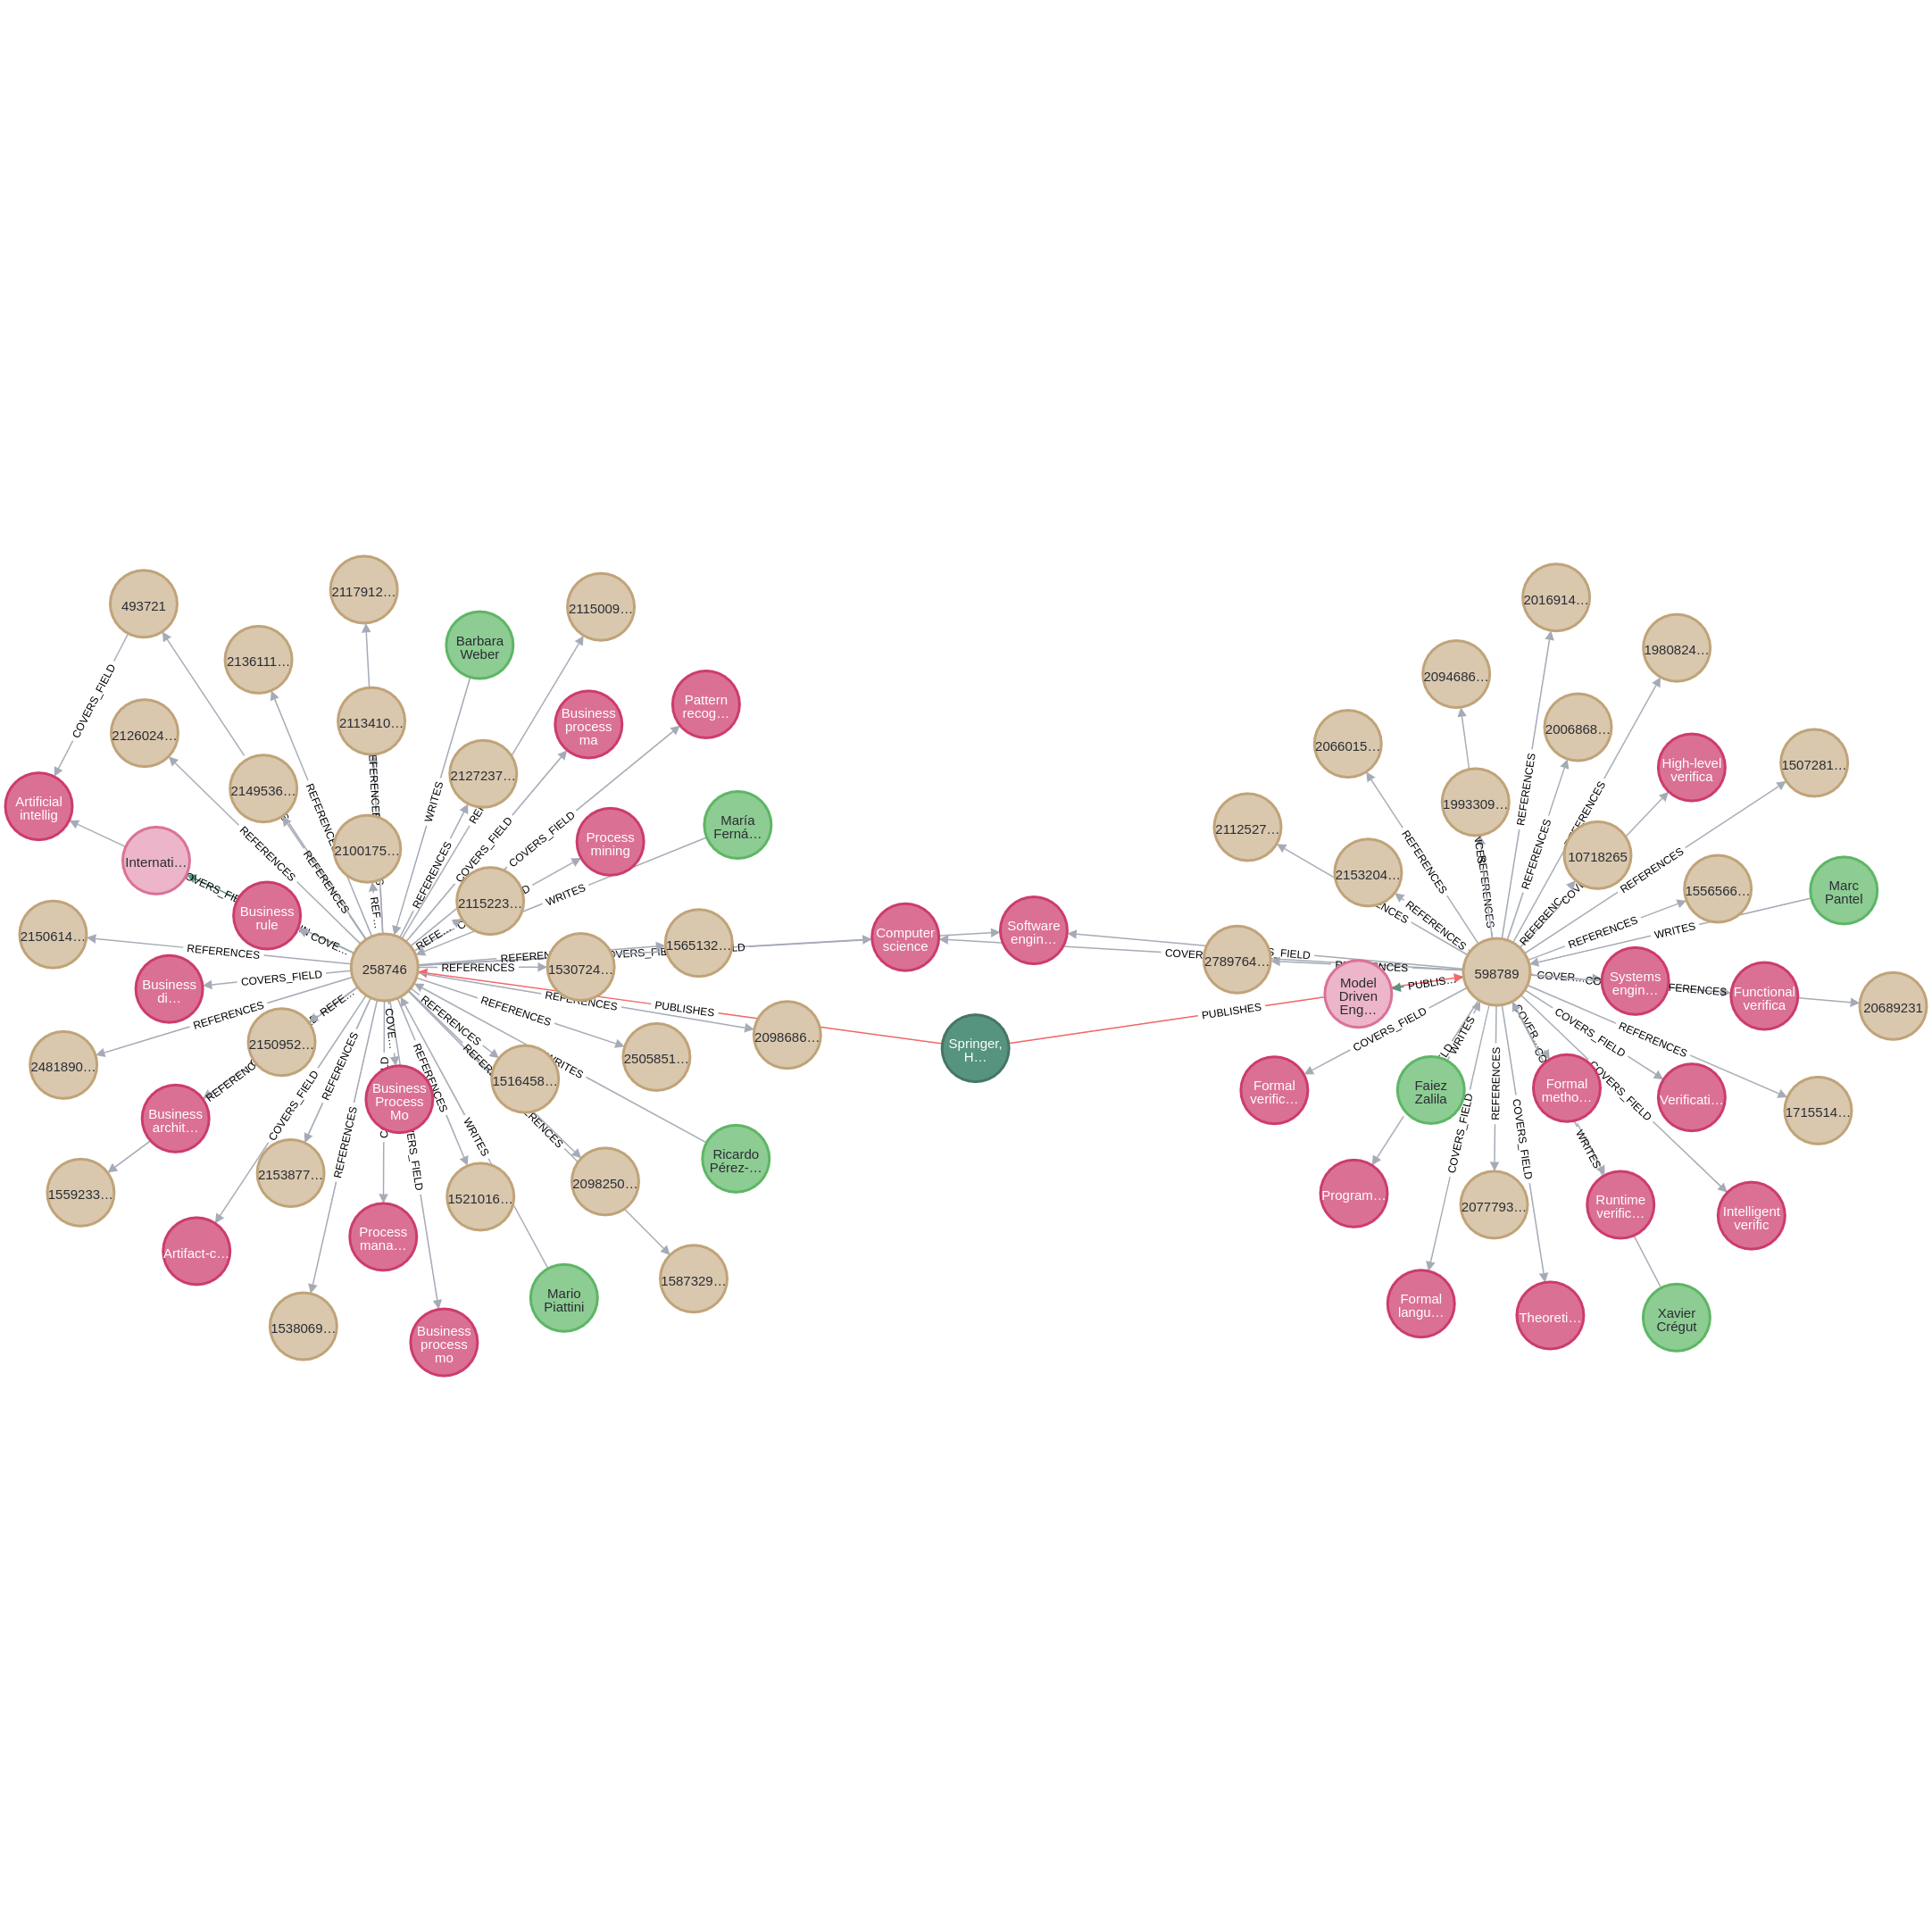
\includegraphics[height=0.5\textwidth]{Images/query_9.png}
        \caption{}
    \label{fig:quadtree}
\end{figure}
\subsection{Find affiliations of the authors who have written the most cited journal publications in the field of Computer Science}

The organizations are the gray nodes, the rest are just for context. \\

\begin{lstlisting}[language=cypher, label=lst:cypher-example]
MATCH (:Journal)<-[:PUBLISHED_IN]-(p:Publication)<-[r:REFERENCES]-(:Publication)
MATCH (p)-[:COVERS_FIELD]->(f:FieldOfStudy)
WHERE f.name = 'Computer science'
WITH COUNT(r) AS citations, p
WITH MAX(citations) AS max_citations
MATCH (:Journal)<-[:PUBLISHED_IN]-(p:Publication)<-[r:REFERENCES]-(:Publication)
WITH COUNT(r) AS citations, p, max_citations
MATCH (o:Organization)<-[:AFFILIATED_TO]-(a:Author)-[:WRITES]->(p)
WHERE citations = max_citations
RETURN DISTINCT o
\end{lstlisting}
\begin{figure}[H]
    \centering
    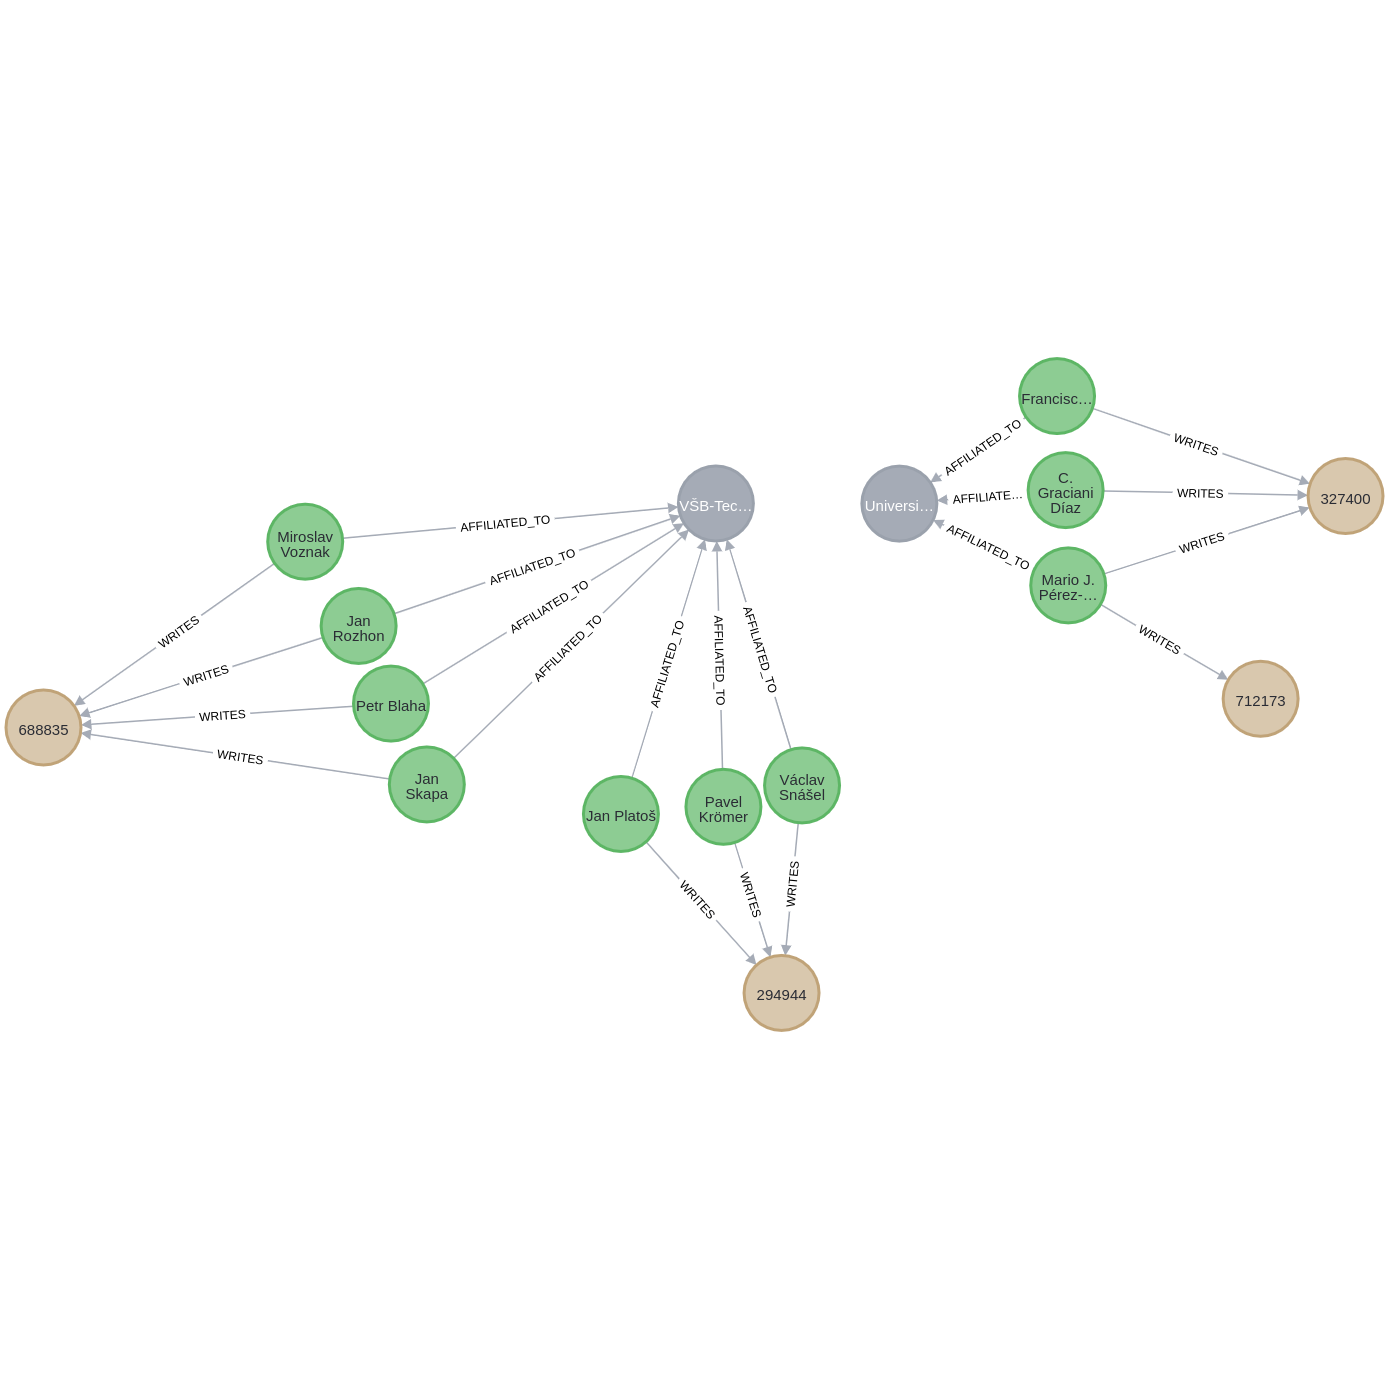
\includegraphics[height=0.5\textwidth]{Images/query_10.png}
        \caption{}
    \label{fig:quadtree}
\end{figure}
\newpage
\subsection{Find the shortest path via citations between two given specific articles (in a given direction)}
We choose a starting article with two possible paths to the other article.
\begin{lstlisting}[language=cypher, label=lst:cypher-example]
MATCH (p:Publication {id: 41593})
MATCH (q:Publication {id: 193006})
MATCH path = shortestPath((q)-[:REFERENCES*]->(p))
RETURN path
\end{lstlisting}
\begin{figure}[H]
    \centering
    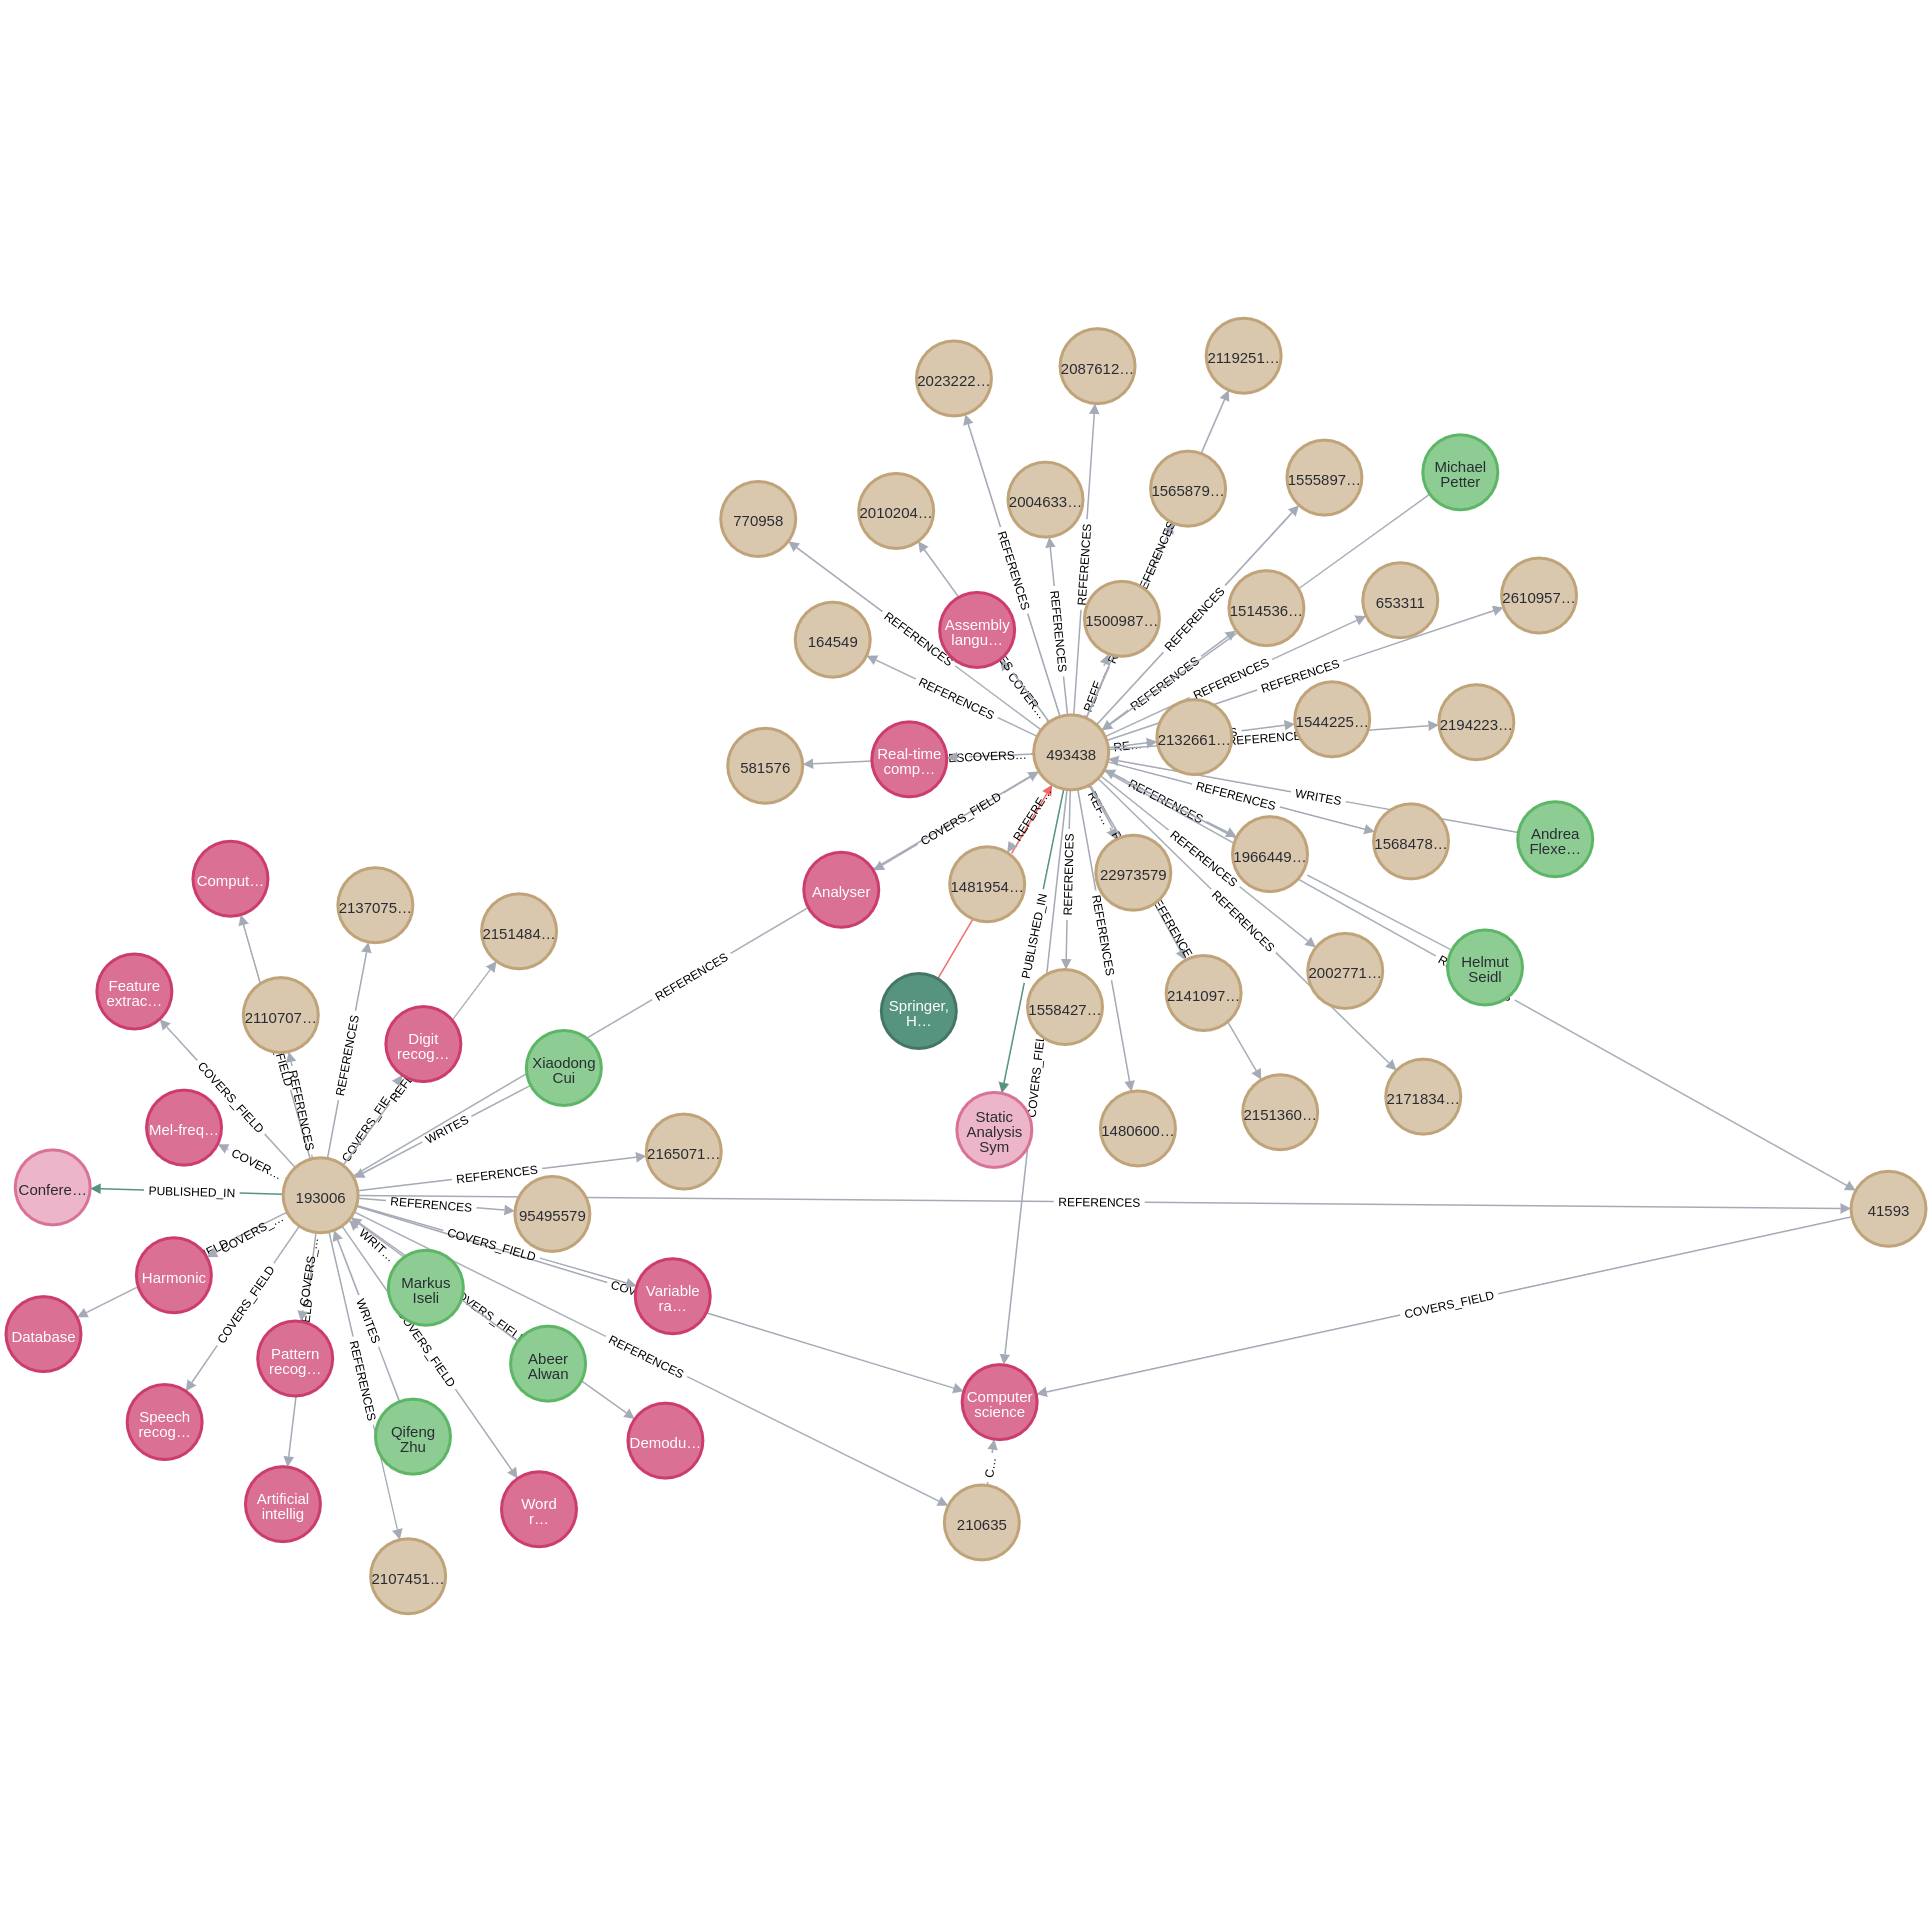
\includegraphics[height=0.5\textwidth]{Images/query_11.png}
        \caption{}
    \label{fig:quadtree}
\end{figure}
Figure 5.16 shows there are two possible paths (expanded). The following figure shows the returned path by \texttt{shortestPath()}.\\
\begin{figure}[H]
    \centering
    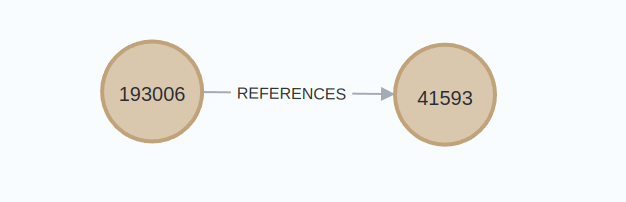
\includegraphics[width=120mm, height=40mm]{Images/query_11_2.png}
        \caption{}
    \label{fig:quadtree}
\end{figure}
\newpage
\subsection{Find the shortest path between two authors, who never have been co-authors. They must have the highest field of study coverage for their publications and the path must be composed of authors and articles.}
First thing is to search for not co-authors.
Then we count separately the field of study covered for each author.
The extraction of the two authors needs another \texttt{MATCH} operation.
Once have the information about the two authors, the shortest path is computed considering only the relations "WRITES" and "REFERENCES". \\
\texttt{LIMIT} is necessary in order to perform the query correctly.\\
\begin{lstlisting}[language=cypher, label=lst:cypher-example]
MATCH (a1:Author)-[:WRITES]->(p1:Publication)-[:COVERS_FIELD]->(f1:FieldOfStudy),
    (a2:Author)-[:WRITES]->(p2:Publication)-[:COVERS_FIELD]->(f2:FieldOfStudy)
WHERE p1 <> p2
WITH DISTINCT count(f1) AS cnt1, count(f2) AS cnt2, a1,a2
WITH max(cnt1) AS field1, max(cnt2) AS field2,a1,a2
MATCH (a1)-[:WRITES]->(p1:Publication)-[:COVERS_FIELD]->(f1:FieldOfStudy),
    (a2)-[:WRITES]->(p2:Publication)-[:COVERS_FIELD]->(f2:FieldOfStudy)
WHERE p1 <> p2
WITH DISTINCT count(f1) AS cnt1, count(f2) AS cnt2, a1,a2,field1,field2
WHERE cnt1 = field1 AND cnt2 = field2
MATCH p = shortestpath((a1)-[*]-(a2))
WHERE all(x IN nodes(p) WHERE "Publication" IN labels(x) OR "Author" IN labels(x))
RETURN p LIMIT 1
\end{lstlisting}
Note that the constrain on co-authors implies "Author 1" and "Author 2" cannot be the same node. \\
\begin{figure}[H]
    \centering
    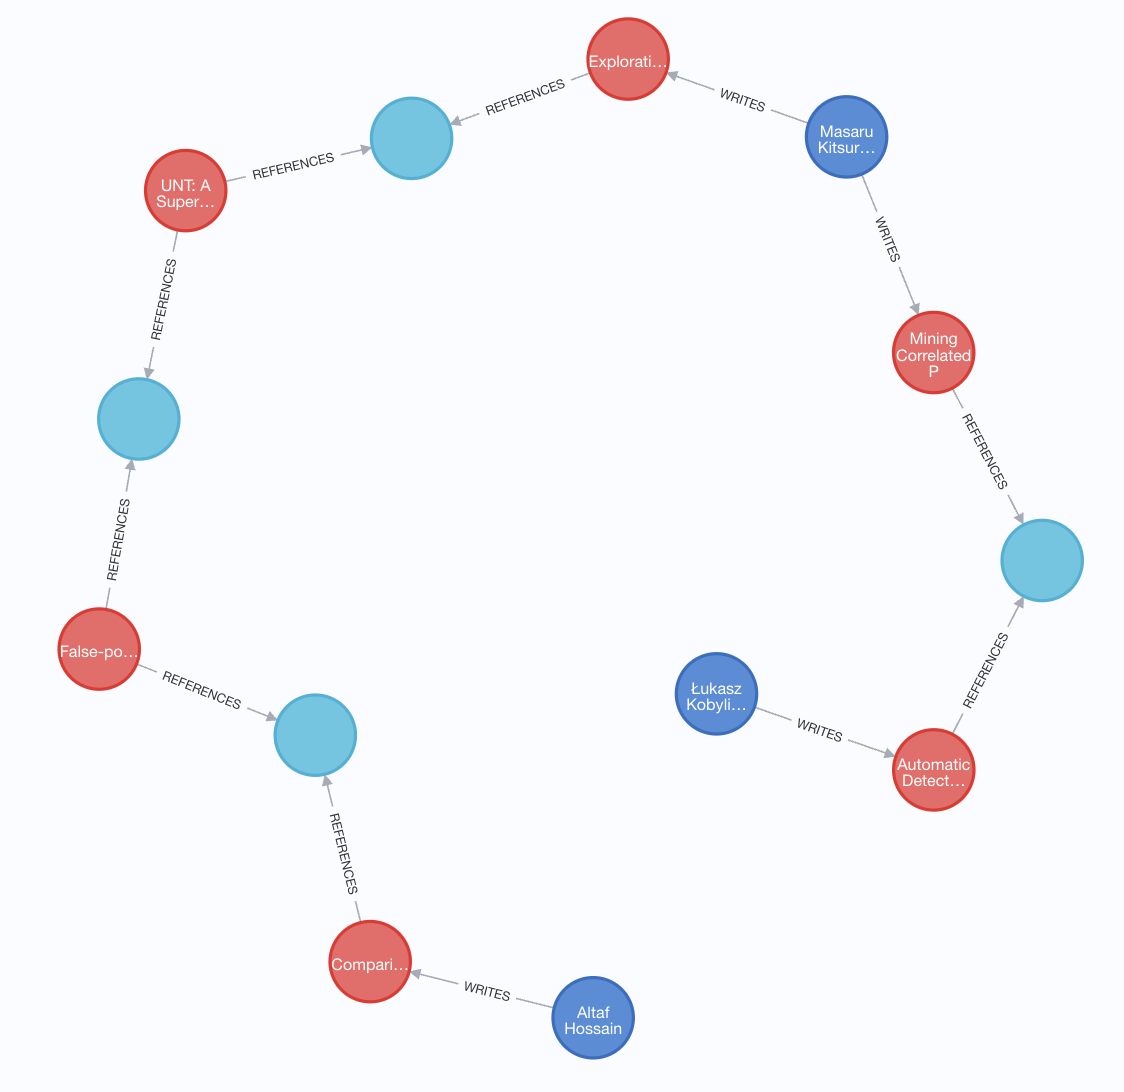
\includegraphics[height=0.44\textwidth]{Images/query_13.png}
        \caption{}
    \label{fig:13}
\end{figure}
\chapter{Performance}
\label{ch:chapter_one}%
\section{Execution Time}
We assess performance by measuring the execution time. Table 6.1 shows the execution time of the queries presented in chapter 5.\\
\begin{table}[H]
\centering 
    \begin{tabular}{|p{4.7em} | c | }
    \hline
    \multicolumn{2}{|c|}{Performance} \\ 
%    \rowcolor{bluepoli!40}
     \hline
      \textbf {Query \#}
     & \textbf{Execution Time (ms)}        \\
    \hline
    \textbf{Query 1} & 2 \\
    \hline
    \textbf{Query 2} & 44 \\
    \hline
    \textbf{Query 3} & 13 \T\B\\
    \hline
    \textbf{Query 4} & 19\T\B\\
    \hline
    \textbf{Query 5} & 9\T\B\\
    \hline
    \textbf{Query 6} & 1241 \T\B\\
    \hline
    \textbf{Query 7} & 5   \T\B\\
    \hline
    \textbf{Query 8} & 10  \T\B\\
    \hline
    \textbf{Query 9} & 11  \T\B\\
    \hline
    \textbf{Query 10} & 3 \T\B\\
    \hline
    \textbf{Query 11} & 12 \T\B\\  
    \hline
    \textbf{Query 12} & 2655 \T\B\\  
    \hline
    \end{tabular}
    \\[20pt]
    \caption{Execution Time}
    \label{table:exampleC}
\end{table}
Queries 6 and 12 have the longest execution times, this is due to checking almost every possible pair of nodes in the database (query 6) and including the comparison among different paths (query 12). 
\end{document}


